
%%%%%%%%%%%%%%%%%%%%%%% file typeinst.tex %%%%%%%%%%%%%%%%%%%%%%%%%
%
% This is the LaTeX source for the instructions to authors using
% the LaTeX document class 'llncs.cls' for contributions to
% the Lecture Notes in Computer Sciences series.
% http://www.springer.com/lncs       Springer Heidelberg 2006/05/04
%
% It may be used as a template for your own input - copy it
% to a new file with a new name and use it as the basis
% for your article.
%
% NB: the document class 'llncs' has its own and detailed documentation, see
% ftp://ftp.springer.de/data/pubftp/pub/tex/latex/llncs/latex2e/llncsdoc.pdf
%
%%%%%%%%%%%%%%%%%%%%%%%%%%%%%%%%%%%%%%%%%%%%%%%%%%%%%%%%%%%%%%%%%%%


\documentclass[runningheads,a4paper]{llncs}

\usepackage{amssymb}
\setcounter{tocdepth}{3}
\usepackage{graphicx}
\usepackage{bm}
\usepackage{multirow}

%\usepackage{url}
%\urldef{\mailsa}\path|{alfred.hofmann, ursula.barth, ingrid.haas, frank.holzwarth,|
%\urldef{\mailsb}\path|anna.kramer, leonie.kunz, christine.reiss, nicole.sator,|
%\urldef{\mailsc}\path|erika.siebert-cole, peter.strasser, lncs}@springer.com|    

\newcommand{\keywords}[1]{\par\addvspace\baselineskip
\noindent\keywordname\enspace\ignorespaces#1}

\begin{document}

\mainmatter  % start of an individual contribution

% first the title is needed
\title{Samsung!}

% a short form should be given in case it is too long for the running head
\titlerunning{Samsung!}


%\thanks{Please note that the LNCS Editorial assumes that all authors have used
%the western naming convention, with given names preceding surnames. This determines
%the structure of the names in the running heads and the author index.}%

% the name(s) of the author(s) follow(s) next
\author{Darya Lavrova, Ruslan Gaisin, Iskander Kareev, Rustem Salimov}
%
\authorrunning{Author running}
% (feature abused for this document to repeat the title also on left hand pages)

% the affiliations are given next; don't give your e-mail address
% unless you accept that it will be published
\institute{Kazan Federal University}
%Springer-Verlag, Computer Science Editorial,\\
%Tiergartenstr. 17, 69121 Heidelberg, Germany\\
%\mailsa\\
%\mailsb\\
%\mailsc\\
%\url{http://www.springer.com/lncs}}

%
% NB: a more complex sample for affiliations and the mapping to the
% corresponding authors can be found in the file "llncs.dem"
% (search for the string "\mainmatter" where a contribution starts).
% "llncs.dem" accompanies the document class "llncs.cls".
%

\toctitle{toc title}
\tocauthor{toc author}
\maketitle


\begin{abstract}
Abstract
\keywords{keywords}
\end{abstract}


\section{Introduction}



\section{Demographic Clusterisation of the Gathered Data}


The investigation was done on the basis of dataset consisting of user's age $x_1$ (column \textit{webapi\_agecateg}), gender $x_2$ (\textit{gender}), marital status $x_3$ (\textit{marital}), occupational status $x_4$ (\textit{jposition}) and infomation on their Internet activity --- the urls which they have visited. 

To improve the robustness of the investigation and clearness of its results we have excluded the urls which were visited with less than 5 users. After the we had total of 526 user entries and 316000 entries on url visits.

Put $U$ to be the set of all users, $S$ to be the set of all sites (urls). By $S(A)$ denote the set of all sites which were visited by at least one user $u \in A \subseteq U$. By $U(s)$ denote the set of all users which visited the site $s \in S$.



\subsection{Clusterization of Users by Demographic Attributes with Control on Diversification of Derived URLs Sets}



On this part of the investigation we have recoded the values in the following way:
\begin{itemize}
\item for values of \textit{marital}: \\ 
	``\textit{Single}''  $\to$ 0,  \quad  ``\textit{In relations}''  $\to$ 0.5, \quad  ``\textit{Married}''  $\to$ 1;
\item for values of \textit{gender}: \\ 
	``\textit{Male}''  $\to$ 0, \quad  ``\textit{Female}'' $\to$ 1;
\item for values of \textit{webapi\_agecateg}: \\ 
	``\textit{0..17}''  $\to$ 1, \quad  ``\textit{18..24}''  $\to$ 2, \quad     ``\textit{25..34}''  $\to$ 3, \quad  ``\textit{35..44}''  $\to$ 4, \quad     ``\textit{45+}''  $\to$ 5;
\item for values of \textit{jposition}: \\ 
	``\textit{employee}'' $\to$ 1, \quad  ``\textit{executive}'' $\to$ 1, \quad  ``\textit{jobless}'' $\to$ 0, \quad  ``\textit{minor}'' $\to$ 0, \quad  ``\textit{student}'' $\to$ 0.5.
\end{itemize}

This allows easy application of classic clusterisation algorithms based on Euclid distance. Here we apply the hierarchic algorithm. The results of clusterisation are highly dependant on the scale of the variables. That is why all the variables were scaled by their means and variances. We bring in a vector of coefficients $\boldsymbol{w} = (w_1, w_2, w_3, w_4), \quad w_i \in [0, 1]$, so rescaled values are supplied to the clusterisation algorithm of the form:
\[
	(w_1 x_1, w_2 x_2, w_3 x_3, w_4 x_4).
\]


\subsubsection{Sites separation measure.}

Let us describe the considered way of choosing of coefficients $\boldsymbol{w}$ values.

Suppose that after the clusterisation with some $\boldsymbol{w}$ the users $U$ are divided on $k$ sets $C_1, C_2, \dots, C_k$:
\[
	C_1 + C_2 + \dots + C_k = U.
\]
Let
\[
	r_{s,j} = \frac{\mathcal{N}(U(s) \cap C_j)}{\mathcal{N}(C_j)}.
\]
By means of $r_{s,j}$ we define an intersection measure for the clusterisation $C_1, C_2, \dots, C_k$:
\[
	M_I(\boldsymbol{w}) = \sum_s \Big( \sum_j r_{s,j} - \min_j \{r_{s,j}\} \Big).
\]

For given number of clusters $k$ we choose the weights $\boldsymbol{w}$ as the ones for which $I(\boldsymbol{w})$ is minimized.



\subsubsection{Clusters number.}

Let $M_I(k) = \min_w M_I(k, \boldsymbol{w})$ be the intersection measure for clustering into $k$ clusters. Fig. illustrates the dependance of the number of unique sites in each group and the value of $M_I$ on value of $k$.

\begin{figure}\label{N7Jti}

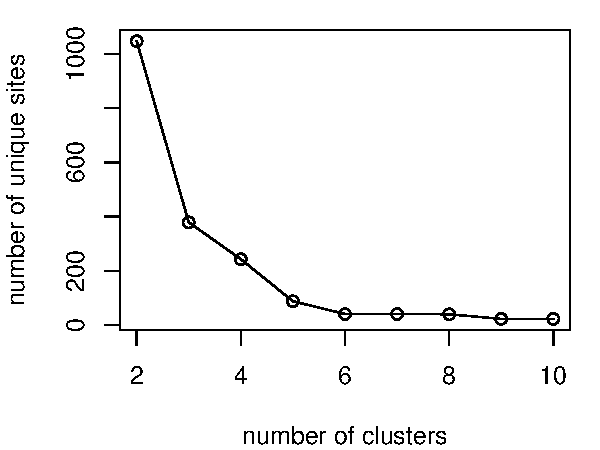
\includegraphics[scale=0.6]{fig_uurls.pdf}\hfill
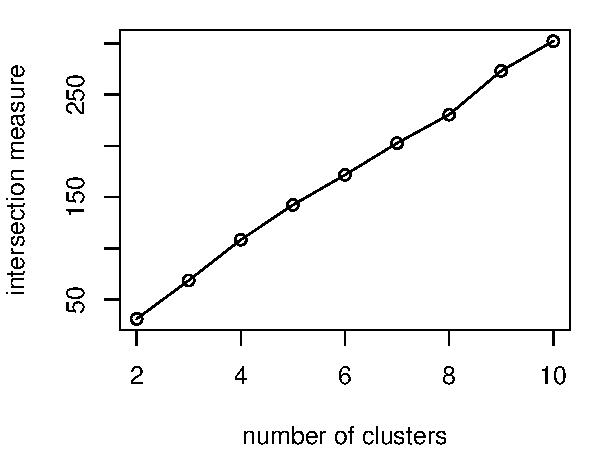
\includegraphics[scale=0.6]{fig_meas.pdf}

\caption{tru-la-la}
\end{figure}

After the AIC algorithm results we chose $k=6$ as the clusters number. For this the weights minimizing the interception measure $M_I$:
\[
	\boldsymbol{w} = (0.4, 0.4, 1.0, 0.4).
\]
On that values of weights we might suggest that the age (to which correspond the weight $1.0$) has the most has the most distinguishing effect on the visiting Internet sites.


\subsubsection{The results.}



\begin{table}\label{OWoti}
	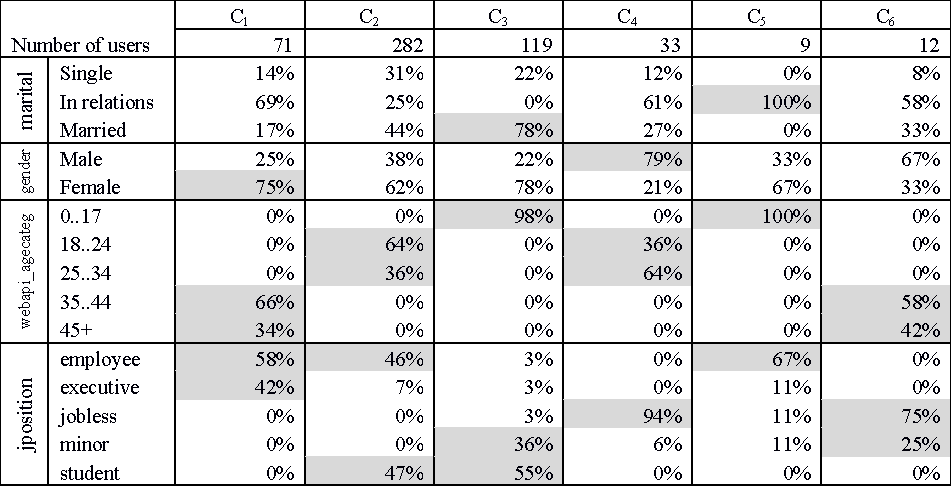
\includegraphics[width=\linewidth]{t1.pdf}
	
	\caption{asd}
\end{table}



\begin{table}\label{01Yti}
	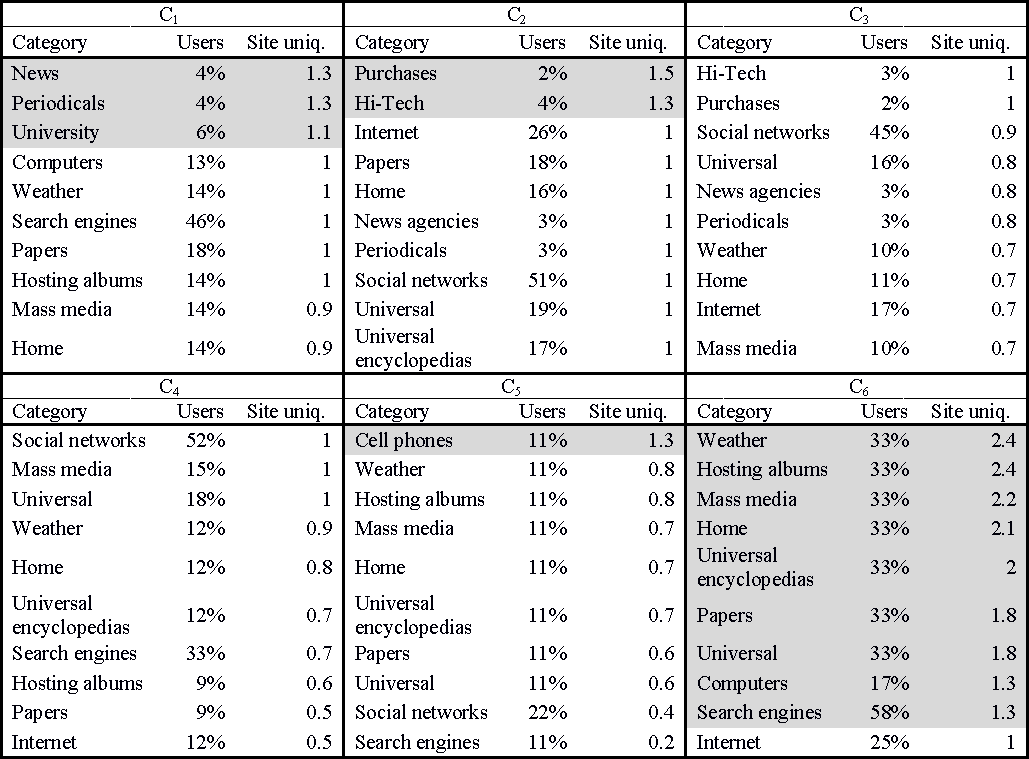
\includegraphics[width=\linewidth]{t2.pdf}
	
	\caption{asd}
\end{table}





\subsubsection*{Acknowledgments.} The heading should be treated as a
subsubsection heading and should not be assigned a number.

\begin{thebibliography}{4}

\bibitem{jour} Smith, T.F., Waterman, M.S.: Identification of Common Molecular
Subsequences. J. Mol. Biol. 147, 195--197 (1981)

\bibitem{lncschap} May, P., Ehrlich, H.C., Steinke, T.: ZIB Structure Prediction Pipeline:
Composing a Complex Biological Workflow through Web Services. In: Nagel,
W.E., Walter, W.V., Lehner, W. (eds.) Euro-Par 2006. LNCS, vol. 4128,
pp. 1148--1158. Springer, Heidelberg (2006)

\bibitem{book} Foster, I., Kesselman, C.: The Grid: Blueprint for a New Computing
Infrastructure. Morgan Kaufmann, San Francisco (1999)

\bibitem{proceeding1} Czajkowski, K., Fitzgerald, S., Foster, I., Kesselman, C.: Grid
Information Services for Distributed Resource Sharing. In: 10th IEEE
International Symposium on High Performance Distributed Computing, pp.
181--184. IEEE Press, New York (2001)

\bibitem{proceeding2} Foster, I., Kesselman, C., Nick, J., Tuecke, S.: The Physiology of the
Grid: an Open Grid Services Architecture for Distributed Systems
Integration. Technical report, Global Grid Forum (2002)

\bibitem{url} National Center for Biotechnology Information, \url{http://www.ncbi.nlm.nih.gov}

\end{thebibliography}




\end{document}
